\input sys/inputs.tex
\usepackage[slovak]{babel}

\begin{document}

\bigheading{Lyžovanie}

% \info{task_name}{infile}{outfile}{points}{timelimit}{memlimit}
% leave this values, if you are not interested
\info{skiing}{stdin}{stdout}{100}{1000 ms}{1 GB}

Programovanie je ťažké, konkurencia silná. Nečudo, že niektorí ľudia to nezvládnu
a dajú sa na inú kariérnu dráhu. Po neúspešnom pokuse o miesto v IOI reprezentácii
sa Kleofáš rozhodol, že radšej bude robiť lyžiarsky slalom. Zajtra má svoj prvý
veľký deň v kariére: Ide prvýkrát na reálne preteky!

Ako iste mnohí viete, súťažná dráha pozostáva z $n$ bránok rozmiestnených po
zasneženom kopci. Súťažiaci potrebuje čo najrýchlejšie prejsť cez všetky bránky a do cieľa.
Nebojte sa, Kleofáš má tajný plán, ako vyhrať. Pôjde po najkratšej možnej trase,
ktorá prejde cez všetky bránky. Teda, samozrejme, ak mu pomôžete túto trasu nájsť,
ináč svoju prehru zvalí na vás.

\heading{Úloha}

Súťažná trať pozostáva z počiatočného bodu $S$, koncového bodu $F$ a $n$ bránok.
Každá bránka je úsečka rovnobežná s osou $x$ (čiže horizontálna). Žiadne dve bránky
nie sú na tej istej $y$-ovej súradnici (v tej istej výške). Začiatočný bod $S$ sa
nachádza nad každou z bránok, čiže jeho $y$-ová súradnica je väčšia ako $y$-ová
súradnica ktorejkoľvek z bránok. Koncový bod $F$ sa nachádza pod všetkými bránkami a 
pod štartovacím bodom.

Nájdite najkratšiu lomenú čiaru začínajúcu v bode $S$, končiacu v bode $F$ a prechádzajúcu
cez všetky bránky v poradí \textbf{zhora nadol}. Lomená čiara prechádza bránkou práve vtedy,
keď majú aspoň jeden spoločný bod. Tento bod \textbf{môže} byť aj krajným bodom bránky.

\heading{Vstup}

Prvý riadok vstupu obsahuje číslo $n$ ($0 \leq n \leq 10^6$) -- počet bránok.
Druhý riadok obsahuje štyri čísla, $x_S, y_S, x_F, y_F$: súradnice bodov $S = (x_S, y_S)$
a $F = (x_F, y_F)$.

Nasleduje $n$ riadkov, $i$-ty z nich obsahuje tri čísla ${x_1}_i, {x_2}_i, {y}_i$ popisujúce $i$-tu
bránu ako úsečku z bodu $({x_1}_i, y_i)$ do bodu $({x_2}_i, y_i)$. Pre každé $i$ platí nerovnosť
${x_1}_i < {x_2}_i$.

Všetky súradnice sú celé čísla medzi $-10^9$ a $10^9$ vrátane. Bránky sú usporiadané zhora
nadol, čiže $y_S > y_1 > y_2 > \dots > y_n > y_F$.

\heading{Výstup}

Dá sa dokázať, že existuje jednoznačná najkratšia lomená čiara spĺňajúca zadanie a vrcholy tejto
čiary majú celočíselné súradnice. Vypíšte lomenú čiaru ako postupnosť vrcholov, v ktorých sa
mení jej smer (nevypisujte zbytočné vrcholy).

\begin{center}
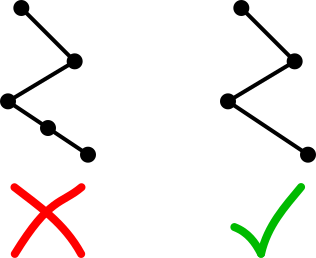
\includegraphics[width=5cm]{img/skiing1}
\end{center}

V prvom riadku výstupu vypíšte číslo $k$, počet vrcholov v optimálnej lomenej čiare. Ďalej vypíšte
$k$ riadkov, v $i$-tom z nich čísla $x_i, y_i$ -- súradnice $i$-teho vrchola čiary. Vrcholy musia
byť vymenované v poradí, v akom idú od začiatku čiary po koniec. To znamená, že musia spĺňať okrem
iného nasledujúce obmedzenia: $x_1 = x_S, y_1 = y_S, x_k = x_F, y_k = y_F$ a $y_1 > y_2 > \dots > y_k$.

\heading{Podúlohy}

\begin{center}
\begin{tabular}{|l|l|l|l|}
\hline
podúloha & počet bodov & maximálne $n$                 \\ \hline
1       & 20     & 200                                          \\ \hline
2       & 30     & 2000                                         \\ \hline
3       & 50     & 1000000                                        \\ \hline
\end{tabular}
\end{center}

\heading{Príklad}


\sampleIN
4
5 10 6 0
0 4 7
7 10 6
5 8 4
2 5 1
\sampleOUT
5
5 10
4 7
7 6
5 1
6 0
\sampleCOMMENT
Situácia vyzerá nasledovne:
\sampleEND
\center{
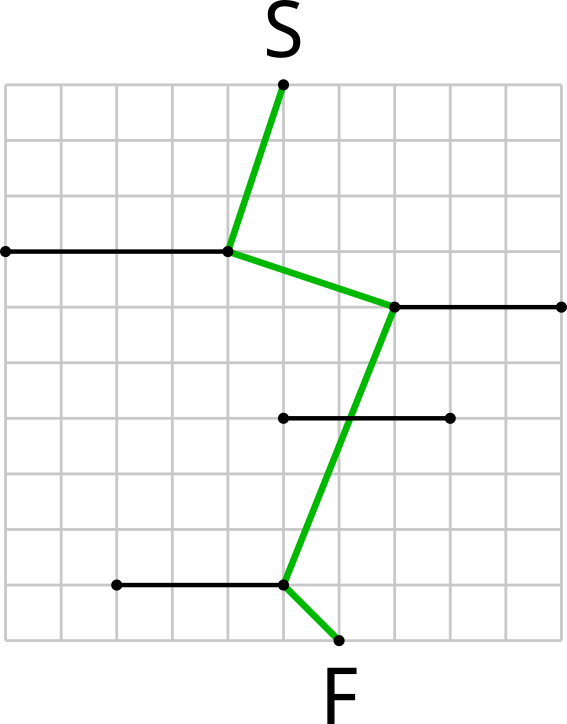
\includegraphics[width=6cm]{img/skiing2}
}

\end{document}
